\lecture[5]{5. Hlutafleiður}{lecture-text}
\date{19.~janúar 2015}
\newcounter{mycount}
\refstepcounter{mycount}

\begin{document}

\subsection{}
	\maketitle






\subsection{Hlutafleiður}
\subsubsection{Skilgreining 5.\arabic{mycount}}\stepcounter{mycount}
 Látum $f(x,y)$ vera fall af tveimur breytum $x$ og $y$ sem er skilgreint á opinni skífu með miðju í punktinum $(a,b)$. 
 
 \medskip
 Skilgreinum \emph{hlutafleiðu m.t.t.} $x$ í $(a,b)$ með
$$f_1(a,b)=\lim_{h\rightarrow 0}\frac{f(a+h,b)-f(a,b)}{h}$$
og {hlutafleiðu m.t.t.} $y$ í $(a,b)$ með
$$f_2(a,b)=\lim_{k\rightarrow 0}\frac{f(a,b+k)-f(a,b)}{k}$$
ef markgildin eru til.





\subsection{Hlutafleiður}
 \begin{figure}[!h]
        \centering
        \begin{minipage}{.5\textwidth}
            \centering
            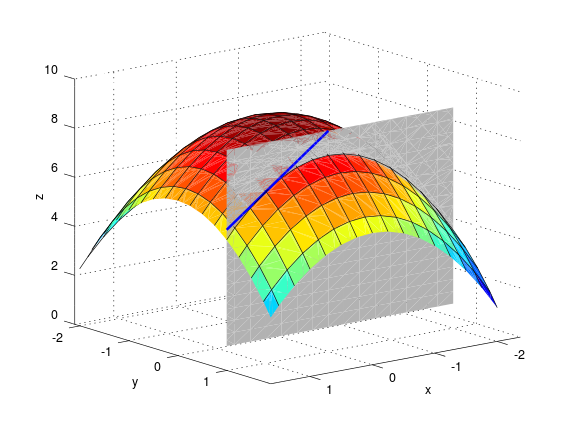
\includegraphics[width=1\linewidth]{xpart.png}
            \caption*{Hlutafleiða m.t.t.~$x$ fyrir $y=1$.}
        \end{minipage}%
        \begin{minipage}{.5\textwidth}
            \centering
            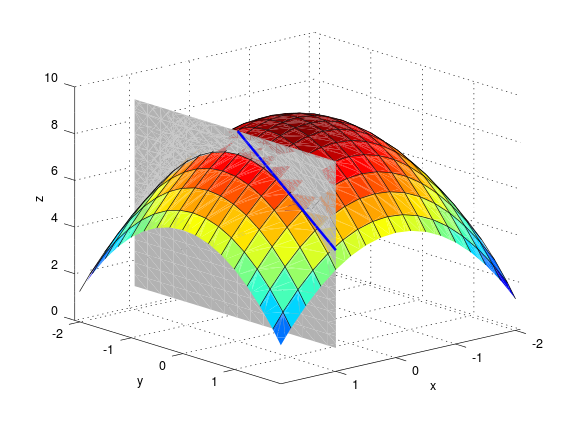
\includegraphics[width=1\linewidth]{ypart.png}
            \caption*{Hlutafleiða m.t.t.~$y$ fyrir $x=1$.}
        \end{minipage}
    \end{figure}
 



\newpage
\subsection{Hlutafleiður}
\subsubsection{Skilgreining 5.\arabic{mycount}}\stepcounter{mycount}
  
Látum $f(x,y,z)$ vera fall af þremur breytum $x$, $y$ og $z$ sem er skilgreint á opinni kúlu með miðju í punktinum $(a, b,c)$. 

\medskip

Skilgreinum \emph{hlutafleiðu m.t.t.} $x$ í $(a,b,c)$ með
$$f_1(a,b,c)=\lim_{h\rightarrow 0}\frac{f(a+h,b,c)-f(a,b,c)}{h},$$
 \emph{hlutafleiðu m.t.t.} $y$ í $(a,b,c)$ með
$$f_2(a,b,c)=\lim_{k\rightarrow 0}\frac{f(a,b+k,c)-f(a,b,c)}{k}$$
og  \emph{hlutafleiðu m.t.t.} $z$ í $(a,b,c)$ með
$$f_3(a,b,c)=\lim_{\ell\rightarrow 0}\frac{f(a,b,c+\ell)-f(a,b,c)}{\ell}$$
ef markgildin eru til.
 






\subsection{Hlutafleiður} 

\subsubsection{Skilgreining 5.\arabic{mycount}}\stepcounter{mycount}
Látum $f$ vera fall af
$n$ breytum $x_1,x_2,\ldots,x_n$ sem er skilgreint á opinni kúlu um punktinn $\mathbf{a}=(a_1, a_2, \ldots, a_n).$ 

\medskip	
{\em Hlutafleiða} $f$ með
tilliti til breytunnar $x_k$ í punktinum $\mathbf{a}$ er skilgreind sem markgildið 
$$f_k(\mathbf{a})=\lim_{h\rightarrow 0}\frac{f(\mathbf{a}+h\ev_k)-f(\mathbf{a})}{h}$$
ef markgildið er til.  (Hér stendur $\ev_k$ fyrir vigurinn sem er með
0 í öllum hnitum nema því $k$-ta þar sem er 1.)








\subsection{}
\Wider{\subsubsection{Ritháttur 5.\arabic{mycount}}\stepcounter{mycount}
   Ritum $z=f(x,y)$.  Ýmis konar ritháttur fyrir hlutafleiður, m.a.~
$$f_1(x,y)=\frac{\partial z}{\partial x}=  \frac{\partial }{\partial x}f(x,y)
=D_1f(x,y)=f_x(x,y)=D_xf(x,y)=\partial_xf(x,y)$$

$$f_2(x,y)=\frac{\partial z}{\partial y}=  \frac{\partial }{\partial y}f(x,y)
=D_2f(x,y)=f_y(x,y)=D_yf(x,y)=\partial_yf(x,y)$$

Þegar við viljum tákna gildið á hlutafleiðu $f$ í ákveðnum punkti
$(x,y)=(a,b)$ þá eru líka ýmsir möguleikar, til dæmis 
$$\frac{\partial z}{\partial x}\bigg|_{(a,b)}=
\left(\frac{\partial }{\partial x}f(x,y)\right)\bigg|_{(a,b)}
=f_1(a,b)=D_1f(a,b)$$
 $$\frac{\partial z}{\partial y}\bigg|_{(a,b)}=
\left(\frac{\partial }{\partial y}f(x,y)\right)\bigg|_{(a,b)}
=f_2(a,b)=D_2f(a,b).$$
 }



\subsection{Snertiplan}
  Látum $f(x,y)$ vera fall af tveimur breytistærðum þannig að hlutafleiðurnar $f_1(a,b)$ og $f_2(a,b)$ séu skilgreindar.
  \begin{figure}
           \centering
            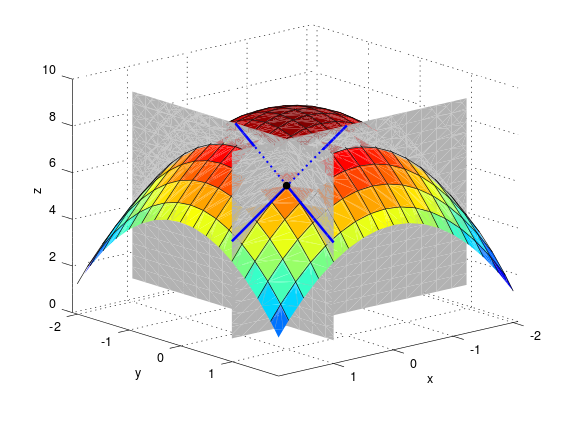
\includegraphics[width=0.6\linewidth]{bothpart.png}
    \end{figure}
    Í punktinum $(a,b,f(a,b))$ er 
    
    $\Tv_1 = \iv + f_1(a,b)\kv\qquad$ snertivigur við ferilinn $f(x,b) = z$ og
    
    $\Tv_2 = \jv + f_2(a,b)\kv\qquad$ snertivigur við ferilinn $f(a,y) = z$.




\subsection{Snertiplan}
 Táknum með $S$ planið sem hefur stikunina
$$(a,b,f(a,b))+s\Tv_1+t\Tv_2, \quad -\infty < s,t < \infty.$$
Vigurinn 
$$\nv=\Tv_2\times \Tv_1=f_1(a,b)\iv+f_2(a,b)\jv-\kv$$
er þvervigur á $S$ og jafna plansins $S$ er
$$z=f(a,b)+f_1(a,b)(x-a)+f_2(a,b)(y-b).$$

\emph{Þverlína} á $S$ hefur stikun
$$(a,b,f(a,b)) + u \nv, \quad -\infty < u < \infty.$$

Ef $f(x,y)$ er 'nógu nálægt' (skilgreint nánar síðar) planinu $S$ þegar $(x,y)$ er nálægt punktinum $(a,b)$ þá kallast $S$ \emph{snertiplan} við grafið $z=f(x,y)$ í punktinum $(a,b,f(a,b)$.


\subsection{Hlutafleiður af hærra stigi}
 \subsubsection{Skilgreining 5.\arabic{mycount}}\stepcounter{mycount}
  Ritum $z=f(x,y)$.  {\em Annars stigs
  hlutafleiður} $f$ eru skilgreindar með formúlunum
$$\frac{\partial^2 z}{\partial x^2}=
\frac{\partial}{\partial x} \frac{\partial z}{\partial x}
=f_{11}(x,y)=f_{xx}(x,y),$$
$$\frac{\partial^2 z}{\partial y^2}=
\frac{\partial}{\partial y} \frac{\partial z}{\partial y}
=f_{22}(x,y)=f_{yy}(x,y),$$
$$\frac{\partial^2 z}{\partial x\partial y}=
\frac{\partial}{\partial x} \frac{\partial z}{\partial y}
=f_{21}(x,y)=f_{yx}(x,y),$$
$$\frac{\partial^2 z}{\partial y\partial x}=
\frac{\partial}{\partial y} \frac{\partial z}{\partial x}
=f_{12}(x,y)=f_{xy}(x,y).$$
Hlutafleiðurnar $f_{11}(x,y)$ og $f_{22}(x,y)$ kallast hreinar
hlutafleiður og $f_{12}(x,y)$ og $f_{21}(x,y)$ kallast blandaðar
hlutafleiður.  
 



\subsection{Hlutafleiður af hærra stigi}
 \subsubsection{Setning 5.\arabic{mycount}}\stepcounter{mycount}
  Látum $f(x,y)$ vera fall sem er skilgreint á opinni
skífu $D$ með miðju í $P=(a,b)$ .  Gerum ráð fyrir að
hlutafleiðurnar $f_1(x,y)$, $f_2(x,y)$, $f_{12}(x,y)$ og $f_{21}(x,y)$
séu allar skilgreindar á $D$ og að þær séu allar samfelldar á $D$.  Þá
gildir að 
$$f_{12}(a,b)=f_{21}(a,b).$$
 



\subsection{Hlutafleiður af hærra stigi}
 \subsubsection{Hugmynd að skilgreiningu 5.\arabic{mycount}}\stepcounter{mycount}
  Skilgreiningu~5.6 má útvíkka á augljósan hátt
til að skilgreina 2.~stigs hlutafleiður fyrir föll af fleiri en
tveimur breytum.   Einnig er augljóst hvernig má skilgreina
hlutafleiður af hærri stigum en 2, til dæmis ef $w=f(x,y,z)$ þá 
$$\frac{\partial^3 w}{\partial x\partial y^2} \quad\quad\mbox{(diffra
    fyrst tvisvar m.t.t. }y\mbox{, svo einu sinni m.t.t. } x\mbox{)}$$
og 
$$\frac{\partial^3 w}{\partial y\partial z\partial y} \quad\quad\mbox{(diffra
    fyrst m.t.t. } y\mbox{, svo m.t.t. } z
\mbox{ og að lokum m.t.t. }y\mbox{)}.$$

 



\subsection{}
 \subsubsection{Setning 5.\arabic{mycount} (Almenn útgáfa af Setningu~5.7)}\stepcounter{mycount}
     Látum $f$ vera
fall $n$ breytistærðum sem er skilgreint á opinni kúlu með miðju í 
$P=(x_1, x_2,\ldots, x_n)$.  

\medskip
Skoðum tvær hlutafleiður $f$ í punktum $P$
þar sem er diffrað með tilliti til sömu breytistærða og jafn oft með
tilliti til hverrar breytistærðar.  Ef þessar hlutafleiður eru
samfelldar í punktinum $P$ og allar hlutafleiður af lægra stigi eru
skilgreindar á $D$ og samfelldar á $D$ þá eru hlutafleiðurnar sem við
erum að skoða jafnar í $P$.
 
\pause
 \subsubsection {Dæmi:} 
 Ef $w = f(x,y,z)$ er fall af þremur breytistærðum þá er t.d.~
 \begin {equation*}
  \frac{\partial^4 w}{\partial x^2\partial y \partial z} = \frac{\partial^4 w}{\partial x \partial y \partial x \partial z}
 \end {equation*}
ef skilyrðin í setningunni eru uppfyllt.
  
 





\end{document}